%!TEX root = doc.tex
%!TEX output_directory = aux

% In the previous section, we provided evidence that the neural network pruning literature suffers from a severe lack of meaningful comparison between methods. In this section, we attempt to shed light on why this is. At a high level, our conclusion is that authors are behaving reasonably given the incentives with which they are presented and the difficulty of performing meaningful comparisons.

% In the previous section, we provided evidence that the neural network pruning literature suffers from a lack of apples-to-apples comparisons between methods. Might it be possible, however, to examine our aggregated results post-hoc and determine which methods are best? The answer appears to be no. In this section, we detail the barriers that we---and authors of pruning papers in general---encounter when attempting to compare existing methods.

% We have already discussed
% In the previous section, we discussed the fragmentation of datasets, models, metrics, and operating points, and how this fragmentation makes implementing controlled comparisons between methods difficult. Regrettably, these difficulties are largely inevitable so long as the literature remains fragmented.

% However, there are some ways in which the barriers to comparison can be lowered. In this section, we focus on preventable obstacles to comparison, which in most cases stem from the presentation and selection of results. In particular, papers often appear to not be written so as to facilitate future comparison to their proposed methods. We discuss several ways in which this manifests and how it increases the difficulty of meaningful comparison between methods. % In the next section, we will also discuss concrete practices to avoid these pitfalls.

In the previous section, we discussed the fragmentation of datasets, models, metrics, operating points, and experimental details, and how this fragmentation makes evaluating the efficacy of individual pruning methods difficult. In this section, we argue that there are additional barriers to comparing methods that stem from common practices in how methods and results are presented.% (or lack thereof) in the literature.

% In particular, papers often appear to not be written so as to facilitate future comparison to their proposed methods. We discuss several ways in which this manifests and how it increases the difficulty of meaningful comparison between methods.

 % a key factor is that many papers are not written with ``forwards compatiblity'' in mind. That is, they appear to not be written so as to facilitate future comparison to their proposed methods. In this section, we discuss several ways in which this manifests and how it increases the difficulty of meaningful comparison between methods.
% In addition to the fragmentation of datasets, models, metrics, and operating points already discussed, a key factor is that many papers are not written with ``forwards compatiblity'' in mind. That is, they appear to not be written so as to facilitate future comparison to their proposed methods. In this section, we discuss several ways in which this manifests and how it increases the difficulty of meaningful comparison between methods.

% % ------------------------------------------------
% \subsection{Practical Barriers}
% % ------------------------------------------------

% % As authors of papers on pruning are no doubt aware, f
% Fairly comparing one's own method to an existing method can require a great deal of work. At best, it requires reimplementing a pruning heuristic within one's own experimental infrastructure. At worst, it requires hooking into another author's source code to attempt---possibly without success---to exactly replicate their experimental conditions. And this is assuming that usable source code is even available. Because different papers use different models, datasets, and experimental setups, this high cost must be paid for each method to which one compares.

% Moreover, even if one has time to write all the needed code, one might still encounter computational limitations. As evidenced by the near total lack of error bars in Figure~\ref{fig:prune_grid}, training or fine-tuning large networks on large datasets is a slow and sometimes expensive process that few authors have the resources to carry out repeatedly. % are willing to carry out more than necessary.

% In short, we believe that authors fail to make many (rigorous) comparisons not for want of desire, but because doing so is extremely difficult. Combined with a review climate in which lackluster evaluations are adequate for even the best conferences, it is unsurprising that the literature has remained in its current state.

% % ------------------------------------------------
% \subsection{Lack of Forwards Compatibility}
% % ------------------------------------------------

% In addition to the practical barriers discussed above, many papers appear to not be written so as to facilitate future comparison to the presented method. In this section, we discuss several ways in which this manifests and how it increases the difficulty of meaningful comparison between methods. % Note that, in the spirit of collegiality, we will in some cases refrain from attributing omissions and mistakes to particular authors.

% % ------------------------------------------------
% % \subsection{Incomplete Characterization of Results}
% \subsection{Incomplete Characterization of Results}
% % ------------------------------------------------

% % As shown in Figure~\ref{fig:prune_grid}, many methods are not comparable because they use different combinations of models, datasets, and metrics, as well as disparate efficiency levels in their efficiency vs accuracy tradeoff curves.
% Recall that a pruning method must balance both efficiency and accuracy, and that this tradeoff can be characterized in terms of a curve of (efficiency, accuracy) pairs associated with a given dataset and model. As we discussed previously, methods with non-overlapping ranges of their reported curves, or with different datasets and models, cannot be directly compared.

% If all papers reported a wide range of points in their tradeoff curves across a large set of models and datasets, there might be some number of direct comparisons between any given pair of methods. %, even if the overall sets of reported results differed.
% % One factor exacerbating this is that authors report few (dataset, architecture) pairs as well as few measurements to characterize each pair's tradeoff curve.
% As we see in the upper half of Figure~\ref{fig:numresults_stats}, however, most papers use at most three (dataset, architecture) pairs; and as we see in the lower half, they use at most three---and often just one---point to characterize each curve. Combined with the fragmentation in experimental choices, this means that different methods' results rarely overlap. Note that the lower half restricts results to the four most common (dataset, architecture) pairs.

% \begin{figure}[h]
% \begin{center}
% 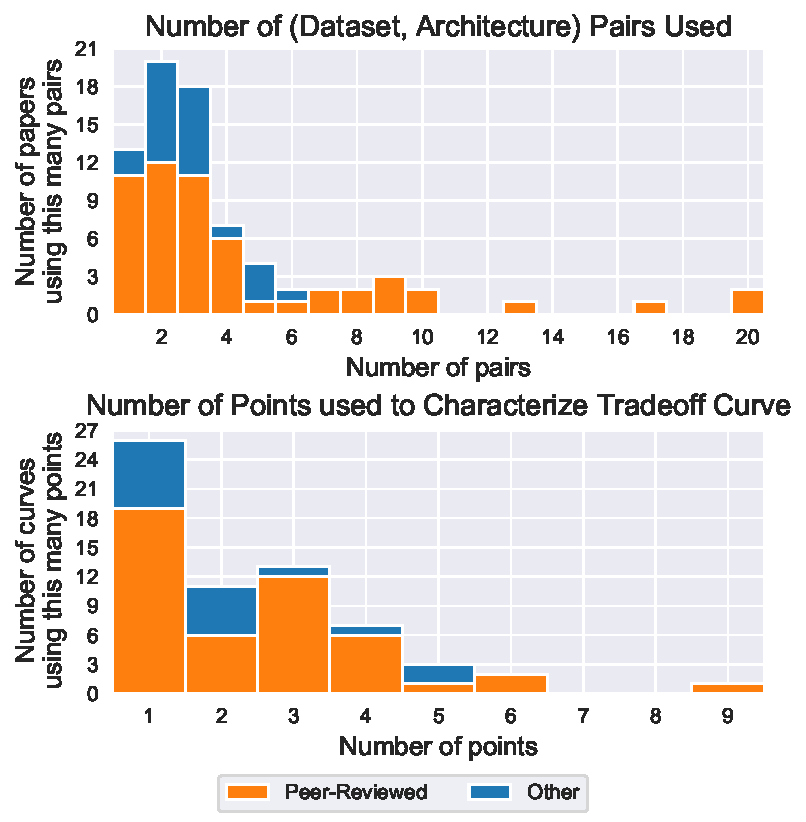
\includegraphics[width=\linewidth]{numresults_stats}
% \caption{Number of results reported by each paper, excluding MNIST. \textit{Top)} Most papers report on three or fewer (dataset, architecture) pairs. \textit{Bottom)} For each pair used, most papers characterize their tradeoff between amount of pruning and accuracy using a single point in the efficiency vs accuracy curve. In both plots, the pattern holds even for peer-reviewed papers.}
% \label{fig:numresults_stats}
% \end{center}
% \end{figure}

% ------------------------------------------------
\subsection{Architecture Ambiguity}
% ------------------------------------------------

It is often difficult, or even impossible, to identify the exact architecture that authors used. Perhaps the most prevalent example of this is when authors report using some sort of ResNet \cite{resnet, resnet2}. Because there are two different variations of ResNets, introduced in these two papers, saying that one used a ``ResNet-50'' is insufficient to identify a particular architecture. Some authors do appear to deliberately point out the type of ResNet they use (e.g., \cite{network-slimming, more-is-less}). However, given that few papers even hint at the possibility of confusion, it seems unlikely that all authors are even aware of the ambiguity, let alone that they have cited the corresponding paper in all cases. % Indeed, at least one paper (\cite{network-slimming}) explicitly mentions using pre-activation ResNets but still cites the other ResNet paper.

% A similar confusion exists for AlexNet \cite{alexnet} vs CaffeNet \cite{caffe, caffenet} and Lenet-5 \cite{lenet} vs Lenet-5-Caffe \cite{lenet-5-caffe}. The second architecture in each case is a slightly different \cite{caffenet, lenet-5-caffe} reimplementation of the first. Even under the optimistic assumption that all authors using these architectures are aware of the differences, it is not always possible to determine from the text what choice they made. For example, \cite{net-surgery, memory-bounded-convnets, ssl}, and \cite{samsung-vbmf-tucker} state that they use Lenet-5 or AlexNet, but mention that they implemented their experiments in Caffe. Since CaffeNet and Lenet-5-Caffe are the default implementations in this framework, it is likely---though unknown---that these authors may have used CaffeNet and Lenet-5-Caffe. A particularly confusing case is the Lenet-5-Caffe reported in \cite{hard-concrete}. The authors are to be commended for explicitly stating not only that they use Lenet-5-Caffe, but the exact architecture they used. However, they describe an architecture with an 800-unit fully-connected layer. Examination of both the Caffe \texttt{.prototxt} files \cite{lenet-5-proto1, lenet-5-proto2} and associated blog post \cite{lenet-5-caffe} indicates that no such layer exists in Lenet-5-Caffe.

Perhaps the greatest confusion is over VGG networks \cite{vgg}. Many papers describe experimenting on ``VGG-16,'' ``VGG,'' or ``VGGNet,'' suggesting a standard and well-known architecture. In many cases, what is actually used is a custom variation of some VGG model, with removed fully-connected layers \cite{google-interchannel, thinet-channel-norms}, smaller fully-connected layers \cite{snip}, or added dropout or batchnorm \cite{network-slimming, snip, extreme-net-compress,sparse-variational-dropout, ding-auto-balanced, apple-pfa}.%, smallify}

% In some cases, the exact variation used is not made clear until the results section, with earlier text suggesting an unmodified ``VGG-16'' \cite{pruning-filters, apple-pfa}. In other cases, the text makes no mention of the particular architecture, with only table headings or contents left to implicitly clarify \cite{eigenDamage, synaptic-strength}. In still others, authors do not directly report what variation they used, but instead indirect to another paper to which they compare. Sometimes this happens recursively. For example, \cite{synaptic-strength} cites \cite{network-slimming} as the source of their model, who in turn attribute their model to a GitHub repository. To add to the confusion, the source code of \cite{network-slimming} documents instead using a variation of this repository's model \cite{slimmingVggSrc}.

% In some cases, the exact variation used is not made clear until the results section, with earlier text suggesting an unmodified ``VGG-16.'' In other cases, the text makes no mention of the particular architecture, with only table headings or contents left to implicitly clarify. In still others, authors do not directly report what variation they used, but instead cite another paper to which they compare.

% Sometimes this happens repeatedly. For example, \cite{synaptic-strength} cites \cite{network-slimming} as the source of their model, who in turn attribute their model to a GitHub repository. To add to the confusion, the source code of \cite{network-slimming} documents instead using a variation of this repository's model \cite{slimmingVggSrc}.
% state ``For our experiment a variation of the original VGGNet for CIFAR dataset is taken from [36]'', where ``[36]'' is

In some cases, papers simply fail to make clear what model they used (even for non-VGG architectures). For example, one paper just states that their segmentation model ``is composed from an inception-like network branch and a DenseNet network branch.'' Another paper attributes their VGGNet to \cite{deepFaceRecognition}, which mentions three VGG networks. \citet{rethinking-net-pruning} and \citet{lottery-ticket} have circular references to one another that can no longer be resolved because of simultaneous revisions. One paper mentions using a ``VGG-S'' from the Caffe Model Zoo, but as of this writing, no model with this name exists there. Perhaps the most confusing case is the Lenet-5-Caffe reported in one 2017 paper. The authors are to be commended for explicitly stating not only that they use Lenet-5-Caffe, but their exact architecture. However, they describe an architecture with an 800-unit fully-connected layer, while examination of both the Caffe \texttt{.prototxt} files \cite{lenet-5-proto1, lenet-5-proto2} and associated blog post \cite{lenet-5-caffe} indicates that no such layer exists in Lenet-5-Caffe.

% net-slimming: "For our experiment a variation of the original VGGNet for CIFAR dataset is taken from [36]", where [36] is torch blog post
% they also refer to stuff as just VGG until clarifying in section 4.2
% also in 4.2 they say "ResNet [14]" where [14] is original resnet paper, but elsewhere they explicitly state that they used  a pre-activation resnet and cite the identity mappings paper

% ------------------------------------------------
\subsection{Metrics Ambiguity} \label{sec:otherAmbiguity}
% ------------------------------------------------

% Though less common than architecture ambiguity, it is not always clear what dataset a paper is using. For example, \cite{lempitsky-cp-decomp} and \cite{openai-block-sparse} don't say what dataset they use with their CharNet and PixelCNN++, respectively. % \cite{more-is-less} provides results for CIFAR-10 and CIFAR

It can also be difficult to know what the reported metrics mean. For example, many papers include a metric along the lines of ``Pruned\%''. In some cases, this means fraction of the parameters or FLOPs remaining \cite{apple-pfa}. In other cases, it means the fraction of parameters or FLOPs removed \cite{learning-both, lempitsky-fast-convnets, balanced-sparsity}. There is also widespread misuse of the term ``compression ratio,'' which the compression literature has long used to mean $\frac{\text{original size}}{\text{compressed size}}$ \cite{bbp, pfor, groupSimd, zfp, dfcm, sprintz}, but many pruning authors define (usually without making the formula explicit) as $1 - \frac{\text{compressed size}}{\text{original size}}$.

Reported ``speedup'' values present similar challenges. These values are sometimes wall time, sometimes original number of FLOPs divided by pruned number of FLOPs, sometimes a more complex formula relating these two quantities \cite{more-is-less, soft-filter-pruning}, and sometimes never made clear. Even when reporting FLOPs, which is nominally a consistent metric, different authors measure it differently (e.g., \cite{nvidia-taylor-pruning} vs \cite{convnet-tensor-decomp}), though most often papers entirely omit their formula for computing FLOPs. We found up to a factor of four variation in the reported FLOPs of different papers for the same architecture and dataset, with \cite{sze-energy-aware} reporting 371 MFLOPs for AlexNet on ImageNet, \cite{samsung-winograd-sparse} reporting 724 MFLOPs, and \cite{learning-both} reporting 1500 MFLOPs.
% , and other papers that give or imply a number reporting 500 MFLOPS.
